\documentclass[12pt,a4paper]{report}
\usepackage[utf8]{vietnam}\usepackage{amsmath, amsthm, amssymb,latexsym,amscd,amsfonts,enumerate}
\usepackage[top=3.5cm, bottom=3.0cm, left=3cm, right=3.0cm]{geometry} 
\usepackage{color, fancyhdr, graphicx, wrapfig}
\usepackage[unicode]{hyperref}
\usepackage[vietnamese]{babel}
\usepackage{titling}
\usepackage{subfigure}
\usepackage{secdot}
\usepackage{enumitem}
\usepackage{array}
\usepackage[tikz]{ocgx2}
\usepackage{xcolor}
\usepackage{tikz}
\usepackage{subcaption}
\usepackage{changepage}
\usepackage{float}
\usepackage{pgfplotstable}
\usepackage{pgfplots}
\usepackage{blindtext}
\usepackage{titlesec}
\usepackage{mathtools}
\usepackage{tabularx}
\usepackage{nccmath}
\usetikzlibrary{calc}
\usepackage{longtable}
\usepackage{indentfirst}
\usepackage{fancyhdr}
\usepackage{exscale,relsize,makeidx}
%\usepackage{refcheck}
\setcounter{tocdepth}{4}
\setcounter{secnumdepth}{4}
\newtheorem{dn}{Định nghĩa}
\newtheorem{tc}{Tính chất}
\newtheorem{dl}{Định lý}
\pgfplotsset{width=7cm, height=6cm}
\newtheorem{md}{Mệnh đề}
\newtheorem{bd}{Bổ đề}
\newtheorem{hq}{Hệ quả}
\newtheorem{nx}{Nhận xét}
\newtheorem{vd}{Ví dụ}
\newtheorem{cy}{Chú ý}
\pagenumbering{roman}\pagestyle{plain}
%\pagestyle{fancy}
%\lhead{\it \changefontsizes{11pt}Luận văn thạc sĩ:}
%\rhead{\it Một số phương pháp vô hướng hóa cơ bản trong tối ưu đa mục tiêu}
%\lfoot{\it Nguyễn Văn Vân } 			         
%\rfoot{\it K19.2 trường ĐHSG}
\renewcommand{\headrulewidth}{1,2pt} 			
\renewcommand{\footrulewidth}{1,2pt}
\newcommand{\dstc}[2]
{
	\newdimen\stringwidth\setbox0=\hbox{#1}
	\stringwidth=\wd0
	\hspace*{-\parindent}\hspace*{.5\textwidth}\hspace*{-.5\wd0}#1\hfill #2\bigskip
	
}  
\usepackage{scrextend}
\fancyhf{}
\lhead{}
\chead{\thepage}
\rhead{}
\cfoot{}
\rfoot{}
\lfoot{}
\pagestyle{fancy}
\usetikzlibrary{patterns}
\renewcommand{\headrulewidth}{1pt}
\begin{document} 
\begin{figure}
    \center
    \begin{tikzpicture}
    \begin{axis}
        [
        xmin=0,xmax=80,
        ymin=0,ymax=80,
        xlabel={$x_1$},
        ylabel={$x_2$},
        grid style={line width=.1pt, draw=darkgray!50},
        major grid style={line width=.2pt,draw=darkgray!50},
        axis lines=middle,
        yticklabel=\empty,
        xticklabel=\empty,
        enlargelimits={abs=0},
        samples=100,
        domain = -10:10,
        ]
        \filldraw[blue!30, pattern=north west lines, pattern color=blue!30, line width=1pt] (300, 250) -- (500, 200) -- (700, 300) -- (700, 500) -- (500, 650) -- (200, 500) -- cycle;
        \node[blue!50] at (600,400) {\tiny $S_F$};
    \end{axis}
    \end{tikzpicture}  
    \caption{Tập nghiệm minh hoạ của bài toán (F)}
    \end{figure}
\begin{figure}
    \center
    \begin{tikzpicture}
    \begin{axis}
        [
        xmin=-10,xmax=80,
        ymin=-10,ymax=80,
        xlabel={$x_1$},
        ylabel={$x_2$},
        grid style={line width=.1pt, draw=darkgray!50},
        major grid style={line width=.2pt,draw=darkgray!50},
        axis lines=middle,
        yticklabel=\empty,
        xticklabel=\empty,
        enlargelimits={abs=0},
        samples=100,
        domain = -20:20,
        ]
        \filldraw[blue!30, pattern=north west lines, pattern color=blue!30, line width=1pt] (300, 250) -- (500, 200) -- (700, 300) -- (700, 500) -- (500, 650) -- (200, 500) -- cycle;
        \node[blue!50] at (600,400) {\tiny $S_F$};
        \node at (200, 250) {\small $F$};
        \node at (200,195) {\large \textbullet};
        \node at (550, -70) {\tiny $D(x)=0$};
        \node[rotate=60] at (420, 700) {\tiny $P(x)=0$};
        \draw (150, 100) -- (500, 800);
        \draw (100, 250) -- (700, -70);
    \end{axis}
    \end{tikzpicture}  
    \caption{Minh hoạ điểm cố định $F$}
\end{figure}
\begin{figure}
    \center
    \begin{tikzpicture}
    \begin{axis}
        [
        xmin=0,xmax=10,
        ymin=0,ymax=15,
        xlabel={$x_1$},
        ylabel={$x_2$},
        grid style={line width=.1pt, draw=darkgray!50},
        major grid style={line width=.2pt,draw=darkgray!50},
        axis lines=middle,
        yticklabel=\empty,
        xticklabel=\empty,
        enlargelimits={abs=0},
        samples=10,
        domain = 0:1,
        ]
        \filldraw[blue!30, pattern=north west lines, pattern color=blue!30, line width=1pt] (0, 0) -- (0, 70) -- (30, 40) -- (40, 20) -- (40, 0) -- cycle;
        \draw (0, 70) -- (70, 0);
        \draw (0, 100) -- (50, 0);
        \draw (40, 0) -- (40, 90);
        \draw[dotted] (0, 80) -- (60, 0);
        \draw[->] (0, 0) -- (15, 20);
        \node at (3, 4) {\tiny O};
        \node at (4, 72) {\tiny C};
        \node at (42, 4) {\tiny E};
        \node at (43, 20) {\tiny G};
        \node at (32, 43) {\tiny K};
        \node at (72, 4) {\tiny D};
        \node at (52, 4) {\tiny B};
        \node at (5, 100) {\tiny A};
        \node at (0, 100) {\tiny \textbullet};
        \node at (0, 70) {\tiny \textbullet};
        \node at (30, 40) {\tiny \textbullet};
        \node at (40, 20) {\tiny \textbullet};
        \node at (40, 0) {\tiny \textbullet};
        \node at (50, 0) {\tiny \textbullet};
        \node at (70, 0) {\tiny \textbullet};
        \node at (0, 0) {\tiny \textbullet};
    \end{axis}
    \end{tikzpicture}  
    \caption{Minh hoạ điểm cố định $F$}
\end{figure}
\begin{figure}
    \center
    \begin{tikzpicture}
    \begin{axis}
        [
        xmin=0,xmax=10,
        ymin=0,ymax=15,
        xlabel={$x_1$},
        ylabel={$x_2$},
        grid style={line width=.1pt, draw=darkgray!50},
        major grid style={line width=.2pt,draw=darkgray!50},
        axis lines=middle,
        yticklabel=\empty,
        xticklabel=\empty,
        enlargelimits={abs=0},
        samples=10,
        domain = 0:1,
        ]
        \filldraw[blue!50, pattern=north west lines, pattern color=blue!90, line width=1.5pt] (0, 0) -- (0, 70) -- (30, 40) -- (40, 20) -- (40, 0) -- cycle;
        \draw (0, 70) -- (70, 0);
        \draw (0, 100) -- (50, 0);
        \draw (40, 0) -- (40, 90);
        \node at (3, 4) {\tiny O};
        \node at (4, 72) {\tiny C};
        \node at (42, 4) {\tiny E};
        \node at (43, 20) {\tiny G};
        \node at (32, 43) {\tiny K};
        \node at (72, 4) {\tiny D};
        \node at (52, 4) {\tiny B};
        \node at (5, 100) {\tiny A};
        \node at (0, 100) {\tiny \textbullet};
        \node at (0, 70) {\tiny \textbullet};
        \node at (30, 40) {\tiny \textbullet};
        \node at (40, 20) {\tiny \textbullet};
        \node at (40, 0) {\tiny \textbullet};
        \node at (50, 0) {\tiny \textbullet};
        \node at (70, 0) {\tiny \textbullet};
        \node at (0, 0) {\tiny \textbullet};
    \end{axis}
    \end{tikzpicture}  
    \caption{Minh hoạ điểm cố định $F$}
\end{figure}
\begin{figure}[!htb]
    \begin{minipage}{0.48\textwidth}
            \center
            \begin{tikzpicture}
            \begin{axis}
                [
                xmin=0,xmax=10,
                ymin=0,ymax=15,
                xlabel={$x_1$},
                ylabel={$x_2$},
                grid style={line width=.1pt, draw=darkgray!50},
                major grid style={line width=.2pt,draw=darkgray!50},
                axis lines=middle,
                yticklabel=\empty,
                xticklabel=\empty,
                enlargelimits={abs=0},
                samples=10,
                domain = 0:1,
                ]
                \filldraw[blue!50, pattern=north west lines, pattern color=blue!90, line width=1.5pt] (0, 0) -- (0, 70) -- (30, 40) -- (40, 20) -- (40, 0) -- cycle;
                \draw (0, 70) -- (70, 0);
                \draw (0, 100) -- (50, 0);
                \draw (40, 0) -- (40, 90);
                \node at (3, 4) {\tiny O};
                \node at (4, 72) {\tiny C};
                \node at (42, 4) {\tiny E};
                \node at (43, 20) {\tiny G};
                \node at (32, 43) {\tiny K};
                \node at (72, 4) {\tiny D};
                \node at (52, 4) {\tiny B};
                \node at (5, 100) {\tiny A};
                \node at (0, 100) {\tiny \textbullet};
                \node at (0, 70) {\tiny \textbullet};
                \node at (30, 40) {\tiny \textbullet};
                \node at (40, 20) {\tiny \textbullet};
                \node at (40, 0) {\tiny \textbullet};
                \node at (50, 0) {\tiny \textbullet};
                \node at (70, 0) {\tiny \textbullet};
                \node at (0, 0) {\tiny \textbullet};
            \end{axis}
            \end{tikzpicture}  
            \caption{Minh hoạ điểm cố định $F$}
    \end{minipage}\hfill
    \begin{minipage}{0.48\textwidth}
            \center
            \begin{tikzpicture}
            \begin{axis}
                [
                xmin=0,xmax=10,
                ymin=0,ymax=15,
                xlabel={$x_1$},
                ylabel={$x_2$},
                grid style={line width=.1pt, draw=darkgray!50},
                major grid style={line width=.2pt,draw=darkgray!50},
                axis lines=middle,
                yticklabel=\empty,
                xticklabel=\empty,
                enlargelimits={abs=0},
                samples=10,
                domain = 0:1,
                ]
                \filldraw[blue!30, pattern=north west lines, pattern color=blue!30, line width=1pt] (0, 0) -- (0, 70) -- (30, 40) -- (40, 20) -- (40, 0) -- cycle;
                \draw (0, 70) -- (70, 0);
                \draw (0, 100) -- (50, 0);
                \draw (40, 0) -- (40, 90);
                \draw[dotted] (0, 80) -- (60, 0);
                \draw[->] (0, 0) -- (15, 20);
                \node at (3, 4) {\tiny O};
                \node at (4, 72) {\tiny C};
                \node at (42, 4) {\tiny E};
                \node at (43, 20) {\tiny G};
                \node at (32, 43) {\tiny K};
                \node at (72, 4) {\tiny D};
                \node at (52, 4) {\tiny B};
                \node at (5, 100) {\tiny A};
                \node at (0, 100) {\tiny \textbullet};
                \node at (0, 70) {\tiny \textbullet};
                \node at (30, 40) {\tiny \textbullet};
                \node at (40, 20) {\tiny \textbullet};
                \node at (40, 0) {\tiny \textbullet};
                \node at (50, 0) {\tiny \textbullet};
                \node at (70, 0) {\tiny \textbullet};
                \node at (0, 0) {\tiny \textbullet};
            \end{axis}
            \end{tikzpicture}  
            \caption{Minh hoạ điểm cố định $F$}
    \end{minipage}
 \end{figure}
 \begin{figure}
    \centering
    \subfigure[]{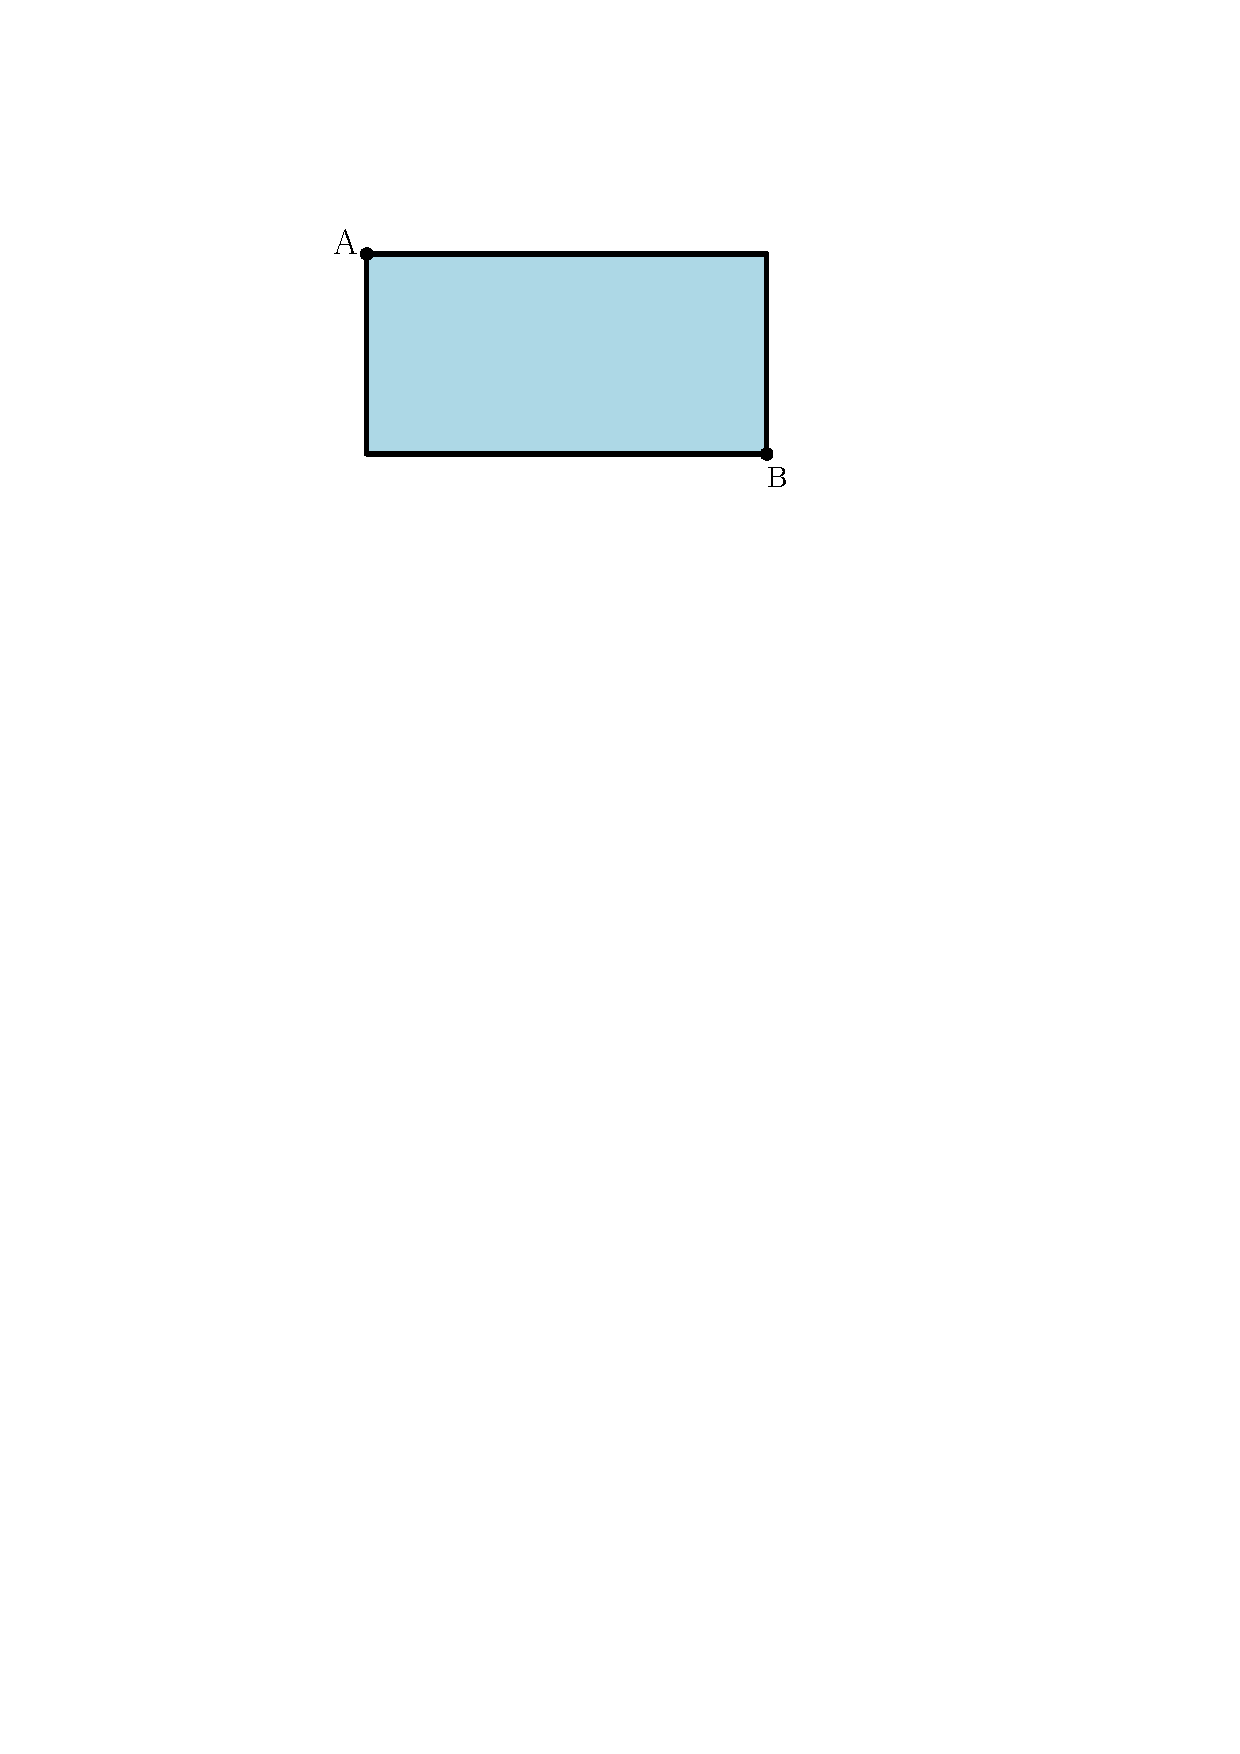
\includegraphics[width=0.2\textwidth]{vuong2.pdf}} 
    \subfigure[]{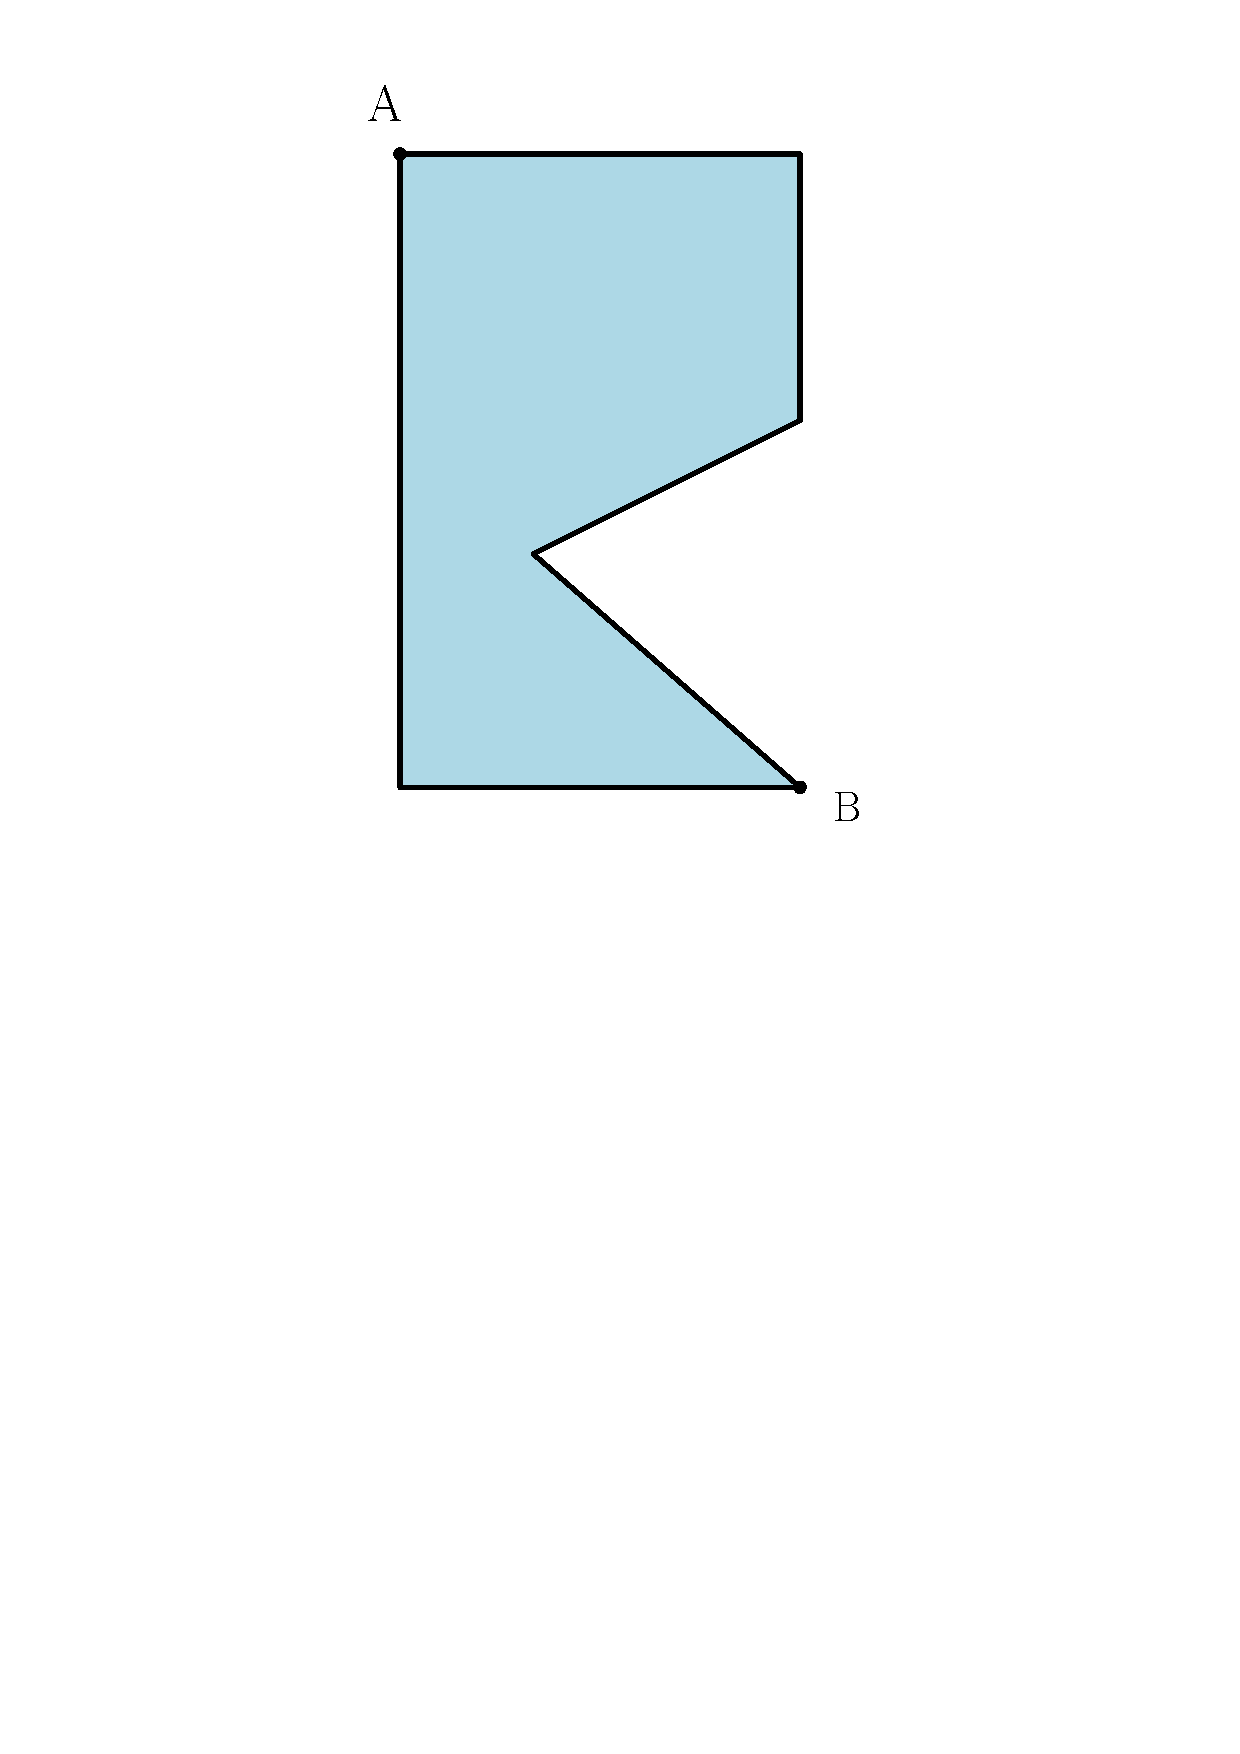
\includegraphics[width=0.15\textwidth]{lom.pdf}} 
    \subfigure[]{
\includegraphics[width=0.15\textwidth]{tron.pdf}} 
    \subfigure[]{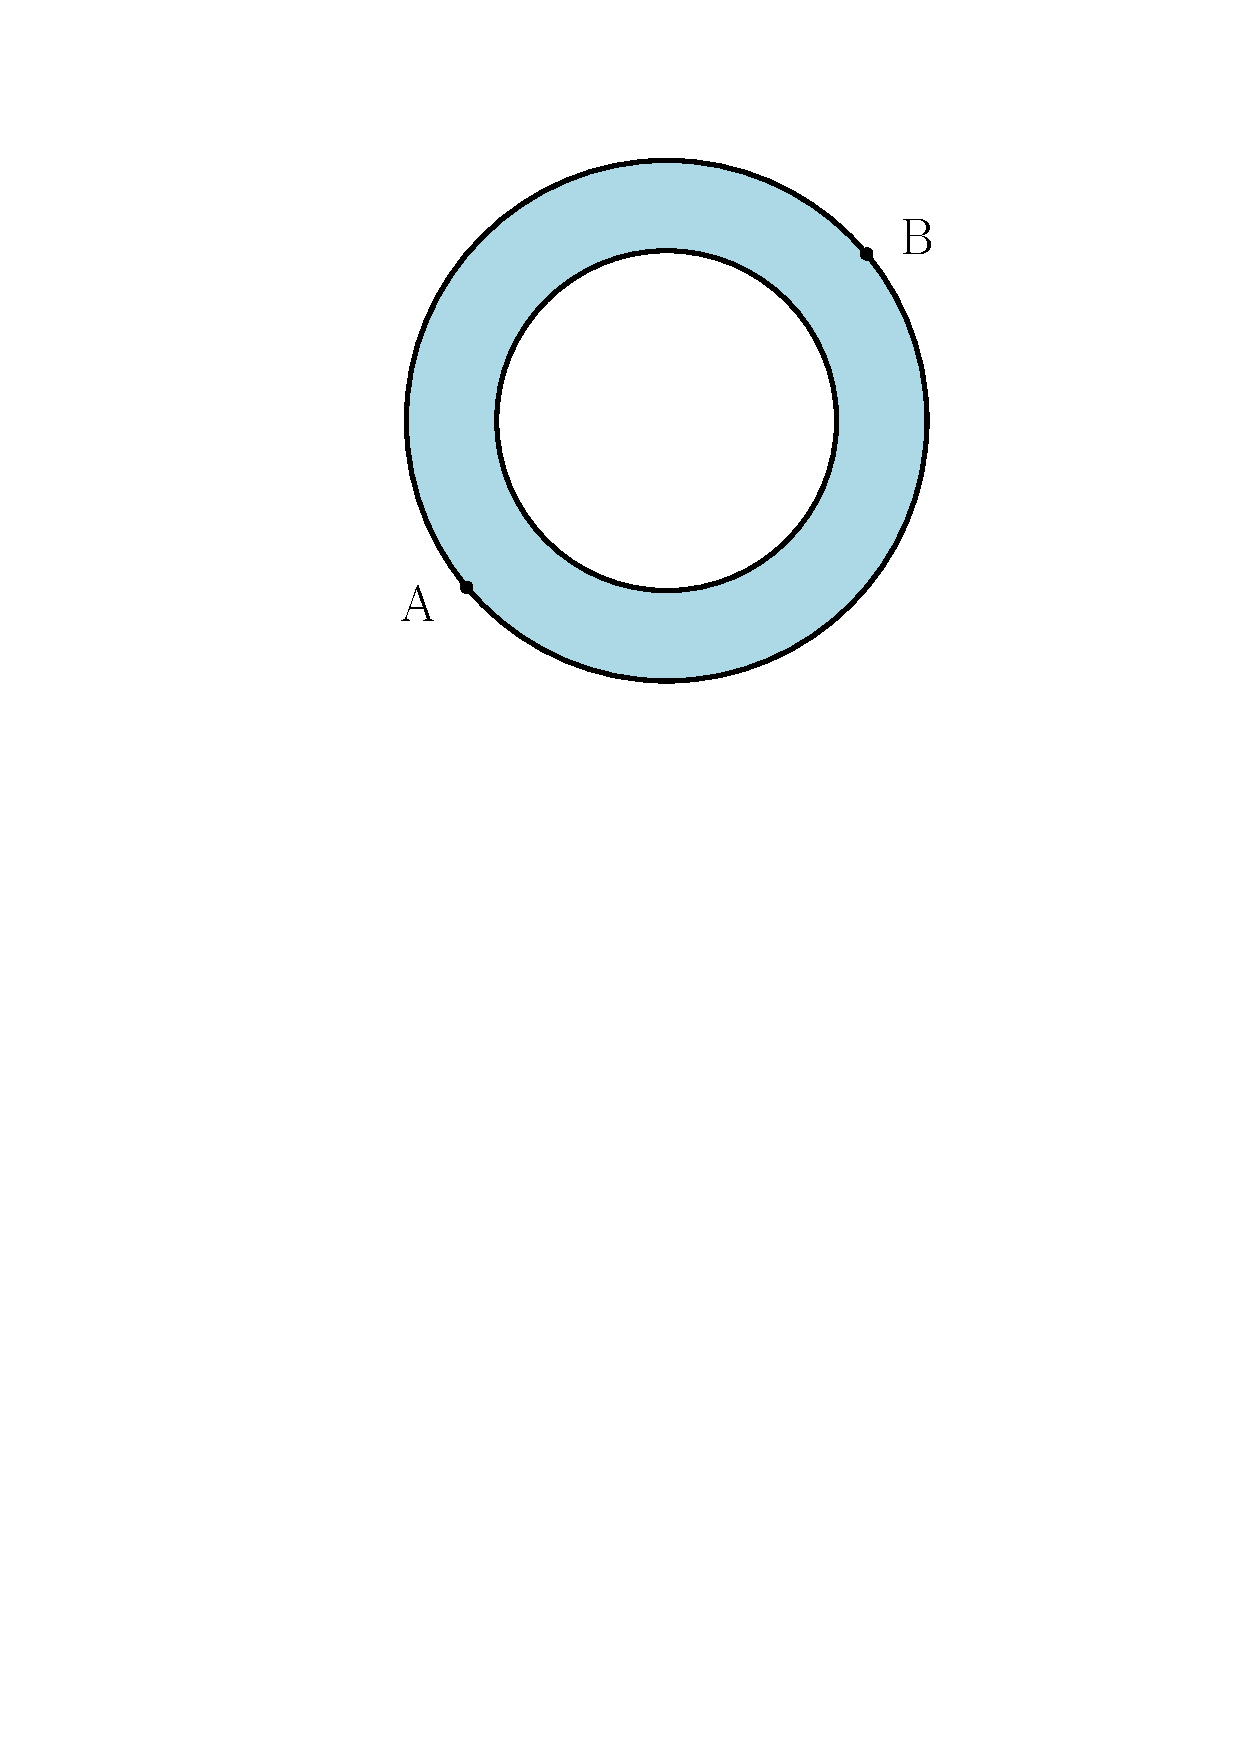
\includegraphics[width=0.15\textwidth]{duc lo.pdf}} 
    \caption{(a) blah (b) blah (c) blah (d) blah}
    \label{fig:foobar}
\end{figure}

\begin{figure}
\end{figure}

\begin{figure}
\end{figure}

\begin{figure}[!htb]
    \begin{minipage}{0.48\textwidth}
    \center
    \begin{tikzpicture}
    \begin{axis}
        [
        xmin=0,xmax=10,
        ymin=0,ymax=15,
        xlabel={$x_1$},
        ylabel={$x_2$},
        grid style={line width=.1pt, draw=darkgray!50},
        major grid style={line width=.2pt,draw=darkgray!50},
        axis lines=middle,
        yticklabel=\empty,
        xticklabel=\empty,
        enlargelimits={abs=0},
        samples=10,
        domain = 0:1,
        ]
        \draw (0, 70) -- (70, 0);
        \draw (0, 100) -- (50, 0);
        \draw (60, 0) -- (60, 90);
        \draw (0, 40) -- (80, 40);
        \node at (3, 4) {\tiny O};
        \node at (4, 72) {\tiny C};
        \node at (32, 45) {\tiny K};
        \node at (72, 4) {\tiny D};
        \node at (52, 4) {\tiny B};
        \node at (5, 100) {\tiny A};
        \node at (0, 100) {\tiny \textbullet};
        \node at (0, 70) {\tiny \textbullet};
        \node at (30, 40) {\tiny \textbullet};
        \node at (50, 0) {\tiny \textbullet};
        \node at (70, 0) {\tiny \textbullet};
        \node at (0, 0) {\tiny \textbullet};
    \end{axis}
    \end{tikzpicture}  
    \caption{Minh hoạ trường hợp bài toán vô nghiệm}
    \end{minipage}\hfill
    \begin{minipage}{0.48\textwidth}
    \center
    \begin{tikzpicture}
    \begin{axis}
        [
        xmin=0,xmax=10,
        ymin=0,ymax=15,
        xlabel={$x_1$},
        ylabel={$x_2$},
        grid style={line width=.1pt, draw=darkgray!50},
        major grid style={line width=.2pt,draw=darkgray!50},
        axis lines=middle,
        yticklabel=\empty,
        xticklabel=\empty,
        enlargelimits={abs=0},
        samples=10,
        domain = 0:1,
        ]
        \filldraw[blue!30, pattern=north west lines, pattern color=blue!30, line width=1pt] (0, 0) -- (0, 70) -- (30, 40) -- (40, 20) -- (40, 0) -- cycle;
        \draw (0, 70) -- (70, 0);
        \draw (0, 100) -- (50, 0);
        \draw (40, 0) -- (40, 90);
        \draw[dotted, line width=2pt] (0, 25.94) -- (13, 0);
        \draw[->] (0, 0) -- (20, 30);
        \node at (3, 4) {\tiny O};
        \node at (4, 72) {\tiny C};
        \node at (42, 4) {\tiny E};
        \node at (43, 20) {\tiny G};
        \node at (32, 43) {\tiny K};
        \node at (72, 4) {\tiny D};
        \node at (52, 4) {\tiny B};
        \node at (5, 100) {\tiny A};
        \node at (0, 100) {\tiny \textbullet};
        \node at (0, 70) {\tiny \textbullet};
        \node at (30, 40) {\tiny \textbullet};
        \node at (40, 20) {\tiny \textbullet};
        \node at (40, 0) {\tiny \textbullet};
        \node at (50, 0) {\tiny \textbullet};
        \node at (70, 0) {\tiny \textbullet};
        \node at (0, 0) {\tiny \textbullet};
    \end{axis}
    \end{tikzpicture}  
    \caption{Minh hoạ trường hợp bài toán có vô số nghiệm}
    \end{minipage}
 \end{figure}

\begin{figure}
    \center
    \begin{tikzpicture}
    \begin{axis}
        [
        xmin=0,xmax=10,
        ymin=0,ymax=15,
        xlabel={$x_1$},
        ylabel={$x_2$},
        grid style={line width=.1pt, draw=darkgray!50},
        major grid style={line width=.2pt,draw=darkgray!50},
        axis lines=middle,
        yticklabel=\empty,
        xticklabel=\empty,
        enlargelimits={abs=0},
        samples=10,
        domain = 0:1,
        ]
        \filldraw[blue!30, pattern=north west lines, pattern color=blue!30, line width=1pt] (0, 200) -- (0, 40) -- (22, 10.5) -- (220, 180) -- cycle;

        \draw (0, 40) -- (30, 0);
        \draw (10, 0) -- (80, 60);
        \draw[->] (0, 0) -- (10, 20);
        \node at (4, 44) {\tiny O};
        \node at (33, 6) {\tiny C};
        \node at (10, 6) {\tiny E};
        \node at (22, 16) {\tiny G};

        \node at (0, 40) {\tiny \textbullet};
        \node at (30, 0) {\tiny \textbullet};
        \node at (10, 0) {\tiny \textbullet};
        \node at (22, 10) {\tiny \textbullet};
    \end{axis}
    \end{tikzpicture}  
    \caption{Minh hoạ điểm cố định $F$}
\end{figure}
\end{document}